\documentclass[12pt,a4paper]{report}
\usepackage{graphicx,wrapfig}
\usepackage{amsmath}
\usepackage{color} % to write text in color
\usepackage{textcomp} %to draw arrow
\graphicspath{ {SVM/SVMimages/} }
\usepackage{setspace}
\doublespacing

\title{Principle Component Analysis}
\author{sumit singh}
\date{October 2017}

\begin{document}

\maketitle
\section{Prologue}
\subsection{Coordinate Axes Transformation}
\begin{figure}[h] \label{Fig:AxisRotation}
\centering
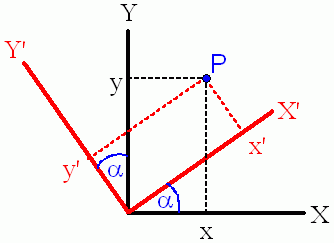
\includegraphics[width = 0.5\textwidth]{SVM/SVMImages/rot_2d_1.png} 
\caption{Rotation of Axis}
\end{figure}
As shown in Figure \ref{Fig:AxisRotation} \\
\begin{align*}
x^{'} &= x \ cos \alpha + y \ sin \alpha \\
y^{'} &= -x \ sin \alpha + y \ cos \alpha 
\end{align*}
Let the polar coordinates of $P$ be $(r,\theta)$, which implies that $x = r Cos\theta $ and $y = r Sin \theta$. Which also implies that $x' = r Cos(\theta -\alpha ) $ and $y = r Sin (\theta - \alpha)$. Expanding the later and then substituting the former gives the above result. \\
\subsection{Sum of Independent Random Varaibles}
[Source: Ross]. \\
\begin{align*}
F_{X+Y}(a) &=  P \{ X+Y \leq a \} \\
&= \iint_{x+y \leq a} f_X(x) f_Y(y) \;  dx dy \\
&= \int_{-\infty}^{\infty} \int_{-\infty}^{a-y} f_X(x) f_Y(y) \; dx  dy \\
&= \int_{-\infty}^{\infty} \int_{-\infty}^{a-y} f_X(x) \; dx \ f_Y(y) \;  dy \\
&= \int_{-\infty}^{\infty} F_X(a-y)f_Y(y) \; dy
\end{align*}
The cumulative distribution $F_{X+Y}$ is called the \textit{convolution} of the distributions $F_X$ and $F_Y$ (the cumulative distribution function of $X$ and $Y$ respectively). \\
By differentiating the CDF, we obtain the probability density function $f_{X+Y}$ of $X+Y$ given be
\begin{align*}
f_{X+Y}(a) &= \frac{d}{da} \int_{-\infty}^{\infty} F_X(a-y)f_Y(y) \; dy \\
 &= \int_{-\infty}^{\infty} \frac{d}{da}  F_X(a-y)f_Y(y) \; dy \\
 &= \int_{-\infty}^{\infty} f_X(a-y)f_Y(y) \; dy \\
\end{align*}
\subsection{Triangular Distribution}
[Source: Ross]. \\
\noindent
{\color{red} \rule{\linewidth}{0.5mm} } \textit{Sum of two independent uniform random variables} {\color{red} If $X$ and $Y$ are independent random variables, both uniformly distributed on $(0,1)$, calculate the probability density of $X+Y$}. \\
\noindent
{\color{red} \rule{\linewidth}{0.5mm} }
\section{Introduction}
Principal component analysis is a data reduction technique. It was developed by Hotelling in 1933. It reduces the number of dimensions. The new dimensions are orthogonal to each other and they are the principal components. 


\section{Mathematics of PCA}

Let us take a two-dimensional matrix, a data of 2 variables and $n$ observations. Say the scatter plot of the data looks like what is shown in Figure \ref{FigPCA2}. 
\[ X_{n \times 2} = 
\begin{bmatrix}
    x_{11} & x_{12}  \\
    x_{21} & x_{22}  \\
    \vdots & \vdots  \\
    x_{d1} & x_{d2} 
\end{bmatrix}
\]

\begin{figure}[!ht] \label{FigPCA2}
    \centering
    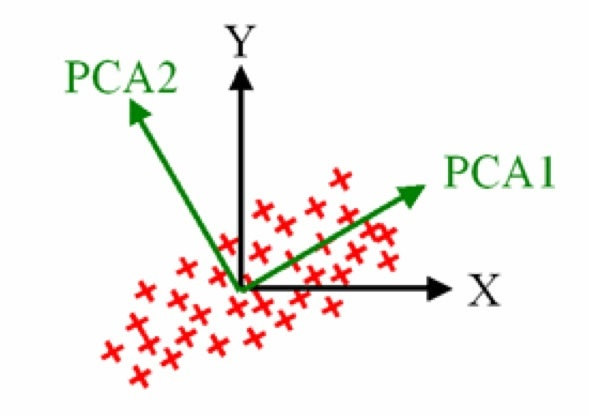
\includegraphics[width = 0.5\textwidth]{SVM/SVMImages/PCA3.jpg}
    \caption{Principal Components in 2-D}
\end{figure}
Let us compute the covariance matrix of $X$ and denote it as:
\[ Cov(X_{1},X_{2}) = 
\begin{bmatrix}
    s_{11} & s_{12}  \\
    s_{21} & s_{22}  
\end{bmatrix}
\]
\begin{figure}[!ht] \label{FigPCA3}
    \centering
    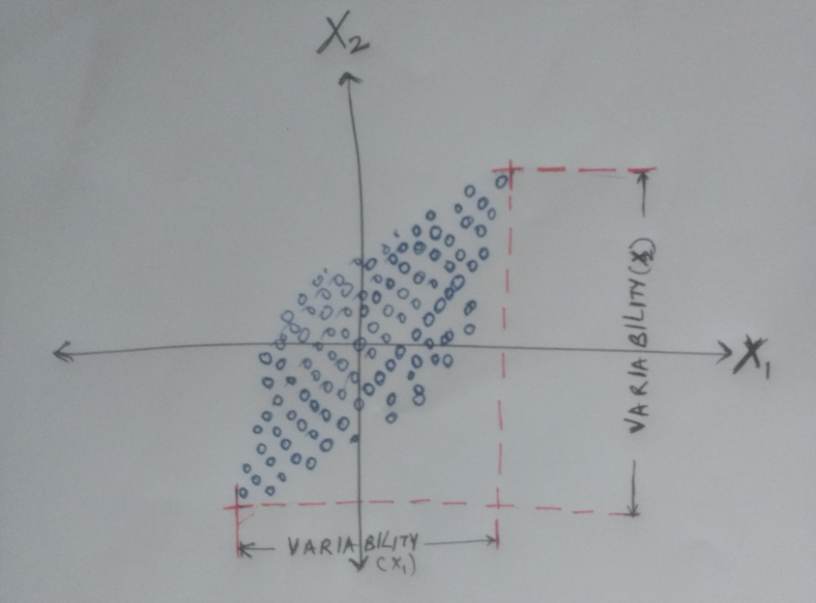
\includegraphics[width = 0.9\textwidth]{SVM/SVMImages/PCA1.PNG}
    \caption{Original Data}
\end{figure}
It is a $2 \times 2$ matrix. The scatter plot shows that there is a relationship between $X_1$ and $X_2$. So, if we calculate the correlation matrix, we will get non zero correlation coefficient.
\[ Corr(X_{1},X_{2}) = 
\begin{bmatrix}
    1 & r_{12}  \\
    r_{21} & 1 
\end{bmatrix}
\]
We know that $-1 \leq r_{12} = r_{21} \leq 1$ and say $r_{12} \cong 0.9$.
The variance of $X_1$ is $s_{11}$ and the variance of $X_2$ is $s_{22}$ which are sample variance. The corresponding population variance matrix is denoted as:

\[ PopulationCov(X) = 
\begin{bmatrix}
    \sigma_{11} & \sigma_{12}  \\
    \sigma_{21} & \sigma_{22}  
\end{bmatrix}
\]
The population variance of $X_1$ is $\sigma_{11}$ and that of  $X_2$ is $\sigma_{22}$. 

As shown in Figure , the variability of $X_1$ and $X_2$ ($s_{11}$ and $s_{22}$ respectively)is not same but they are both high. \\
\begin{figure}[!ht] \label{FigPCA3}
    \centering
    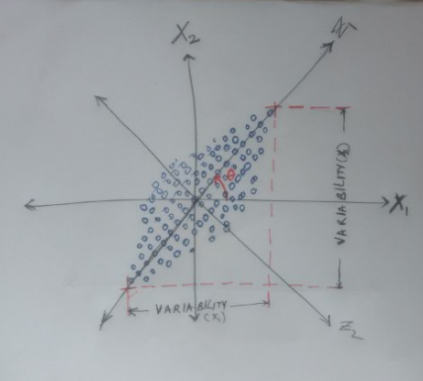
\includegraphics[width = 0.9\textwidth]{SVM/SVMImages/PCA4.PNG}
    \caption{Transformation}
\end{figure}
Now, we rotate the axis ${X_1}$ and ${X_2}$ by an angle $\theta$. Let us call the new axes $Z_1$ and $Z_2$. Now, let us see the variability along the new axes $Z_1$ and $Z_2$. Let us draw a figure along the new axes $Z_1$ and $Z_2$ and call this transformed data. We compare the two diagrams and see that $Variability(Z_1) \gg Variability (X_1)$ and similarly, or rather even more so,  $Variability(Z_2) \ll Variability (X_2)$.\\
\begin{figure}[!ht] \label{FigPCA4}
    \centering
    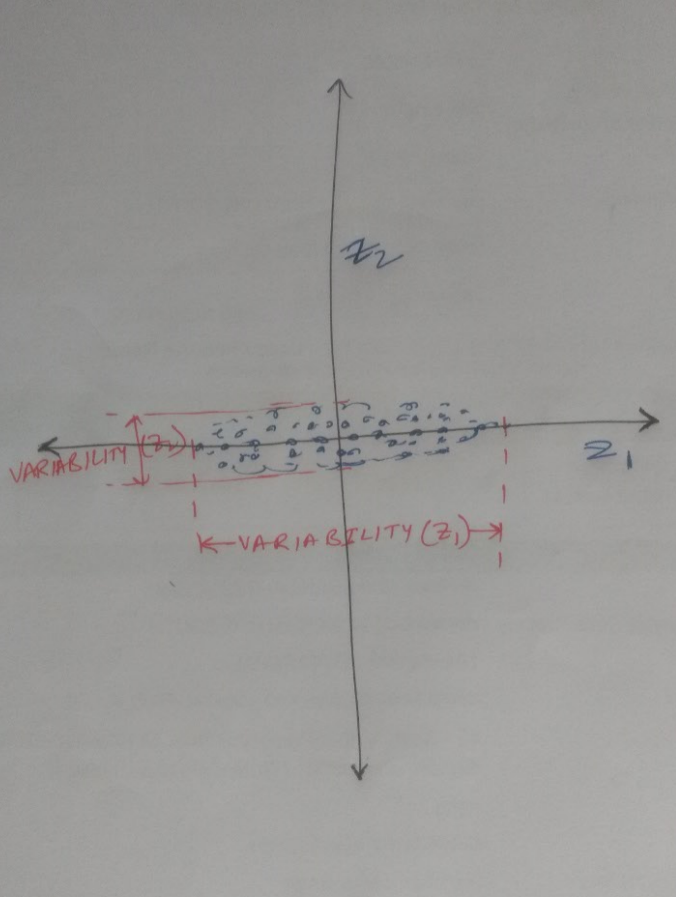
\includegraphics[width = 0.9\textwidth]{SVM/SVMImages/PCA2.PNG}
    \caption{Transformed Data}
\end{figure}
And, in the transformed axes as shown in Fig \ref{FigPCA4}:
\begin{itemize}
\item 
\begin{equation}
V(Z_1) \gg V(Z_2)
\end{equation}
Since the variability across $Z_2$ is much less compared to $Z_1$, then we can say that the information content across $Z_2$ dimension is very less. In fact, we can ignore that information and we can just capture the information along $Z_1$. In statistical sense, \textit{information is nothing but the variability/variance }. $Z_1$ alone is enough to give the information which was scattered all over $X_1$ \& $X_2$. We can in fact ignore the dimension $Z_2$, which will leave us with lesser number of dimension. That is why PCA is essentially a dimensionality reduction technique. The dimension reduction can be done for $p$-dimension matrix as well.\\
\item \underline{Orthogonal Dimensions}.
The major and minor axes of the ellipse (of the scatter plot) is parallel to the (transformed) coordinate axes which was not the case earlier in the $X_1$ \& $X_2$ axes system. When the major and minor axes of the ellipse is not parallel to the coordinate axes, it shows a dependency between the axes,  $X_1$ \& $X_2$. That is not the case with the transformed axes  $Z_1$ \& $Z_2$ which shows that they are independent, \textit{that they are orthogonal}. \underline{Orthogonality is preserved}
\end{itemize}
So, we are trying to develop a mathematical formulation where uncorrelated data structure is transformed to an uncorrelated data structure (the axis of the ellipse is parallel to the transformed coordinate axes) in a reduced dimension. \\
A reduction from $p$-dimension to a lesser number of dimension is what PCA does. By p-dimension, it means an $n \times p$ matrix. $p$ denotes the number of variables, the number of columns of data. $n$ denotes the number of observations, number of rows of data:
\[
X
=
\begin{bmatrix}
    x_{11} & x_{12} & x_{13} & \dots  & x_{1p} \\
    x_{21} & x_{22} & x_{23} & \dots  & x_{2p} \\
    \vdots & \vdots & \vdots & \ddots & \vdots \\
    x_{n1} & x_{d2} & x_{d3} & \dots  & x_{np}
\end{bmatrix}
=
\begin{bmatrix}
    X_{1}^T \\
    X_{2}^T \\
    \vdots \\
    X_{p}^T 
\end{bmatrix}

\]
We transform it from $X$ space to $Z$ space.
$X_{n,p}$ $\,\to\,$ $Z_{n,q}$ where $q \ll p$. PCA is a dimensionality reduction technique. It transforms the original data matrix into a reduced components matrix and it preserves the orthogonality of the components. Suppose we want to do a prediction models using multivariate regression. The $X$s are independent variables (IV). If these IVs are correlated, then that would lead to the problem of multicollinearity. The linear model will not work as the determinant of the matrix will be zero. One of the solution to this problem is the ridge regression. But, if we can make them independent by transformations then the variables would be truly independent and then linear regression can be applied. This is one of the advantages of PCA.\\
What is \textit{Principal}? \\
What is the method? we will go by the same $2 \times 2$ matrix, with scatter plot of the data in the shape of ellipse. Let us consider a point at random from all the data points, say $M$ with coordinates $(x_1,x_2)$. The coordinates of the point $M$ on the transformed axis will be (Assuming that $Z_1$ is at angle $\theta$ counter clock wise from $X_1$):
\begin{align}
z_1 &: x_1 cos \theta + x_2 sin \theta \\
z_2 &: -x_1 sin \theta + x_2 cos \theta 
\end{align}
which in mtrix form can be written as: 
\begin{equation}
\begin{bmatrix}
    z_{1} \\
    z_{2}
\end{bmatrix}
=
\begin{bmatrix}
    cos \theta & sin \theta \\
    - sin \theta & cos \theta
\end{bmatrix}
\begin{bmatrix}
    x_{1} \\
    x_{2}
\end{bmatrix}
\end{equation}
or
\begin{equation}
Z =  A^T X
\end{equation}

where,

\begin{equation}
Z = 
\begin{bmatrix}
    z_{1} \\
    z_{2}
\end{bmatrix}
\end{equation} 
\begin{equation}
A = 
\begin{bmatrix}
    cos \theta & -sin \theta \\
     sin \theta & cos \theta
\end{bmatrix}
\end{equation} 
and 
\begin{equation}
X = 
\begin{bmatrix}
    x_{1} \\
    x_{2}
\end{bmatrix}
\end{equation}
Now, if instead of $p=2$ we have $p=p$, we will get:\\
\begin{equation}
Z = 
\begin{bmatrix}
    z_{1} \\
    z_{2} \\
    \vdots \\
    z_{p} 
\end{bmatrix}
= 
\begin{bmatrix}
    a_{11} & a_{12} & \dots  & a_{1p} \\
    a_{21} & a_{22} & \dots  & a_{2p} \\
    \vdots & \vdots & \ddots & \vdots \\
    a_{p1} & a_{p2} & \dots  & a_{pp}
\end{bmatrix}
\begin{bmatrix}
    x_{1} \\
    x_{2} \\
    \vdots \\
    x_{p} 
\end{bmatrix}
\end{equation}
In terms of dimensions:
\begin{equation}
Z_{p \times 1} = [A_{p \times p}]^T \times X_{p \times 1}
\end{equation}
We say that it is an orthogonal transformation. Let's see now, how this orthogonality is maintained. Let's see with the two-dimension case.
\begin{equation}
A = 
\begin{bmatrix}
    cos \theta & -sin \theta \\
     sin \theta & cos \theta
\end{bmatrix}
= 
\begin{bmatrix}
    a_1 & a_2 \\
\end{bmatrix}
\end{equation} 

where 

\begin{equation}
a_1 = 
\begin{bmatrix}
    cos \theta  \\
     sin \theta 
\end{bmatrix}
\end{equation} 

and 
\begin{equation}
a_2 = 
\begin{bmatrix}
    -sin \theta  \\
    cos \theta 
\end{bmatrix}
\end{equation} 
Now, 
\begin{equation}
a_1^T a_1 =
\begin{bmatrix}
    cos \theta  & sin \theta 
\end{bmatrix}
\begin{bmatrix}
    cos \theta  \\
     sin \theta 
\end{bmatrix}
=
1
\end{equation}

Similarly,

\begin{equation}
a_2^T a_2 = 1
\end{equation}

Now,

\begin{equation}
A^T A = 
\begin{bmatrix}
    cos \theta & sin \theta \\
    -sin \theta & cos \theta
\end{bmatrix}
\begin{bmatrix}
    cos \theta & -sin \theta \\
     sin \theta & cos \theta
\end{bmatrix}
\end{equation}

\begin{equation}
\implies
A^T A = 
\begin{bmatrix}
    1 & 0 \\
    0 & 1
\end{bmatrix}
= A A^T
= A^{-1} A
\end{equation}

\begin{equation}
\implies
A^{-1} A = 
I
\end{equation}
which means, $A$ is an orthogonal matrix, the off diagonal elements are $0$. This shows that the transformation that we are doing is an orthogonal transformation. \textit{$A$ is an orthogonal transformation matrix}.\\

In case of $p$ variables:
\begin{align}
z_1 &= a_1^T x = a_{11}X_1 + a_{12}X_2 + \dots + a_{1p}X_p \\
z_2 &= a_2^T x = a_{21}X_1 + a_{22}X_2 + \dots + a_{2p}X_p \\
\vdots &= \dots = \dots \quad  \dots \quad \dots \quad \dots \quad \dots   \\
z_j &= a_j^T x = a_{j1}X_1 + a_{j2}X_2 + \dots + a_{jp}X_p \\
\vdots &= \dots = \dots \quad  \dots \quad \dots \quad \dots \quad \dots  \\
z_p &= a_p^T x = a_{p1}X_1 + a_{p2}X_2 + \dots + a_{pp}X_p 
\end{align}
where,
\begin{equation}
a_j^T a_j = 1, \quad j = 1,2, \dots, p
\end{equation}
and 

\begin{equation}
var(z_1) \geq var(z_2) \geq \dots \geq var(z_p) 
\end{equation}
We want the first principal component in such a manner that it will explain the maximum variance possible. Second principal component will explain the next maximum variance followed (after taking into account the variance already explained by the first principal component) and so on and so forth. \\
Now, the next step is, how to extract the principal components given the data matrix $X$. \\
The $j^{th}$ principal component, $Z_j$ is equal to $a_j^t x$. So,
\begin{equation}
Var(Z_j) = Var(a_j^t x) =a_j^t Var( x) a_j
\end{equation}
as $a_j$ is a constant vector.
\begin{equation}
Var(X) = Cov(X) = \Sigma = 
\begin{bmatrix}
    \sigma_{11} & \sigma_{12} & \dots  & \sigma_{1p} \\
    \sigma_{21} & \sigma_{22} & \dots  & \sigma_{2p} \\
    \vdots & \vdots & \ddots & \vdots \\
    \sigma_{p1} & \sigma_{p2} & \dots  & \sigma_{pp}
\end{bmatrix}

\end{equation}
as $X$ is multivariate data.

\begin{equation}
\implies Var(Z_j) = a_j^t \Sigma a_j
\end{equation}

Now,

\begin{equation}
E[Z_j] = E[a_j^T x] = a_j^T  E[x] = a_j^T  \mu
\end{equation}

\begin{equation}
a_j^T x \sim (a_j^T  \mu , a_j^t \Sigma a_j)
\end{equation}
If it is Normally distributed, then,
\begin{equation}
a_j^T x \sim N (a_j^T  \mu , a_j^t \Sigma a_j)
\end{equation}

$\Sigma$ and $\mu$ are population parameters. If they are known, then it is population principal component analysis. But, it is usually unknown. In such a case $\overline X$ is used as the best estimate of $\mu$ and $S$, the sample covariance matrix, is used as the estimate for $\sigma$. And, in that case the PCA is known as sample principal component analysis. Since population parameters are rarely known, we will be going ahead with sample PCA.
In sample PCA:
\begin{equation}
E[z_j] = E[a_j^T X] = a_j^T E[X] = a_j^T  \overline X
\end{equation}
\begin{equation}
Var(z_j) = Var(a_j^T X) = a_j^T Cov(X) a_j = a_j^T S a_j  
\end{equation}
If it is normally distributed then,

\begin{equation}
a_j^T \sim ( a_j^T  \overline X, a_j^T S a_j )
\end{equation}
Now, we will look at the principles followed to extract the PCs.
Principles of Principals:
\begin{itemize}
\item Each PC  is a linear combination of $X$, a $p \times 1 $ variable vector, i.e., $a_j^T X$
\item First PC is $a_1^T X$, subjected to $a_1^T a_1 = 1$ that maximizes $Var(a_1^T X)$
\item Second PC is $a_2^T X$ that maximizes $Var(a_2^T X)$ and  subjected to $a_2^T a_2 = 1$  and $Cov(a_1^T X, a_2^T X) = 0$
\item The $j^{th}$ PC is  $a_j^T X$ that maximizes $Var(a_j^T X)$ and subjected to $a_j^T a_j = 1$  and $Cov(a_j^T, a_k^T X) = 0$ for $k < j$
\end{itemize}
$Var(Z_1)$ is the maximum variance in the data and $a_1^T a_1 = 1$. $Var(Z_2)$ is the maximum variance in the data after $Var(Z_1)$ has been removed and $a_2^T a_2 = 1$ and $cov(a_1 X, a_2 X ) = 0$. Since the components are orthogonal, therefore $cov(a_1 X, a_2 X ) = 0$. $Var(Z_3)$ is the maximum variance in the data after $Var(Z_1)$ and $Var(Z_2)$has been removed and $a_3^T a_3 = 1$ and $cov(a_1 X, a_3 X ) = 0$, $cov(a_2 X, a_3 X ) = 0$. And so on and so forth. \\
Now, the optimization problem is :
 $Maximize \quad Var(Z_j) = Maximize \quad a_j^T S a_j$ subject to $a_j^T  a_j = 1$ which can be written as $a_j^T  a_j - 1 = 0$.\\
 Using Langragian:
 \begin{equation}
 Max \quad \mathcal L = a_j^T S a_j - \lambda (a_j^T  a_j - 1)
 \end{equation}
 
 where $\lambda$ is the lagrange multiplier. We need to find the value of $a_j$ such that $\mathcal L $ is maximized. Using First Order Condition, 
 \begin{equation}
 \frac{\partial \mathcal L}{\partial a_j} = 0
 \end{equation}

 \begin{align}
  \implies 2 S a_j -2 \lambda a_j & = 0 \\
 \implies (S - \lambda I) a_j & = 0
 \end{align}
 $S$ is a matrix and $\lambda$ is a scalar hence the identity matrix $I$. S is a $p \times p $ matrix as their are $p$ variables. $\lambda$ is a scalar. $I$ is a  $p \times p $ identity matrix. $|S - \lambda I| = 0$ is the characteristic equation. If $S$ is a $p \times p $ matrix, then the characteristic equation has $p$ roots which will be $\lambda_1 \geq \lambda_2 \geq \dots \geq \lambda_p $. The  $\lambda$s are the eigen values and the corrsponding eigen vectors give the values of the corresponding principals $a_j$. Each of the eigen value is the variance along the corresponding dimension. 



\end{document}